\documentclass{article}
\usepackage[utf8]{inputenc}
\usepackage[norsk]{babel}
\usepackage{makeidx}
\usepackage{circuitikz}
\usepackage{multicol}
\usepackage[margin=3cm]{geometry}
\usepackage{graphicx}
\usepackage{wrapfig}
\usepackage{amsmath}

\graphicspath{ {images/} }

% Dark theme
\usepackage{xcolor}
\pagecolor[rgb]{0.16,0.17,0.2}
\color[rgb]{1,1,1}

\title{Rapport Lab 4}
\author{Johannes Tomren Røsvik og Jon Ryfetten}
\date{\today}

\makeindex

\begin{document}
\pagenumbering{gobble}

% FORSIDE
\begin{titlepage}
	\centering
	{\Large TFE4102 Krets og digitalteknologi \par}
	\vfill
	{\Large Rapport\par}
	\vspace{0.5cm}
	{\huge\bfseries Lab 4\par}
	{\huge\bfseries Absoluttverdi 4-bit\par}
	\vfill
	{av\par}
	{\Large Jon Ryfetten\par}
	{\Large Johannes Tomren Røsvik\par}
	\vspace{1cm}
	{\large Labgruppe 15 \par}
	\vfill
	{\large Lab utført: 15. mars 2017 \par}
	{\large Lab levert: \today \par}
	\vfill
	{FAKULTET FOR INFORMASJONSTEKNOLOGI OG ELEKTROTEKNIKK \par}
\end{titlepage}

% TITTELSIDE
\begin{titlepage}
	\centering
	{.\par}
	\vspace{7cm}
	{\huge\bfseries Absoluttverdi 4-bit \par}
	\vfill
\end{titlepage}

\newpage
% SAMMENDRAG
Raporten er basert på hva som ble gjort i lab 4 den 15. mars 2017. Den omhandlet oppkobling og design av en 4-bit absoluttverdi krets. Basert på XOR og AND porter i ferdig brett var oppgaven å koble dette opp slik at man kunne ta absoluttverdien av en 4-bit binært tall.



% INNHOLDSFORTEGNELSE
\newpage

\tableofcontents{}

\newpage
\pagenumbering{arabic}

\section{Innledning}
I løpet av laboratorieøvingen er målet å lære hvordan absoluttverdikretser kan bygges opp. Man skal også kunne få en forståelse for digitalteknikk med fysiske portkretser. I slutten av laboratorieøvingen ser man også på stige-/falltid og forplatningsforsinkelse.

Øvingen er delt inn i to deler, hvor den første omhandler forarbeid og den neste arbeid utført i laben. I all hovedsak handler mye av forarbeidet på å forstå og designe 4-bit absoluttverdi kretsen. Den praktiske delen er mer blanet.
\newpage
\section{'Teoridelen'}
\subsection{Absoluttverdi}
Uavhengig av tallsystem, så handler absoluttverdi om å omforme et tall slik at det alltid er positivt. Når det kommer til binære tall, så har man forskjellige type representasjoner. De mest vanlige er magnitude med og uten fortegn samt toerkomplement. Det er først når man kommer til toerkomplement at det blir en utfordring å ta absoluttverdi.

For å ta absoluttverdien av et negativt tall på toerkomplement form må man invertere alle bitsene i tallet og deretter legge til en’. Man må også ta hensyn til at positive tall, disse skal ikke gjøres noe med. Man kan finne ut om et tall på toerkomplement form er negativt ved å lese den mest signifikante bitsen. Om det er null impliserer dette at tallet er positivt.

\subsection{Invertering av bits}
For å invertere bitsene kan man bruke en krets bygget opp av XOR-porter. Hver port tar inn in bit samt den mest signifikante bit. Av sannhetstabellen [..] kan vi se at XOR-porten vil invertere A når B er høy, ellers vil utgangen være lik A.

\begin{table}[h]
	\centering
	\caption{XOR-sannhetstabell}
	\label{my-label}
	\vspace{0.2cm}
	\begin{tabular}{| c | c | c |} \hline
		A & B & Q \\ \hline
		0 & 0 & 0 \\ \hline
		0 & 1 & 1 \\ \hline
		1 & 0 & 1 \\ \hline
		1 & 1 & 0 \\ \hline
	\end{tabular}
\end{table}

\subsection{Ripple Carry}
For å kunne legge til en’ i et binært tall kan man bruke en «Ripple Carry»-adderer. Adderen har som formål å kunne addere to binære tall. Denne baser seg på at man har en blokk for hver bit. Hver av blokkene legger sammen tre bit. En carry, samt et tall med lik indeks fra hver av input tallene. «Carry»-biten kommer fra sist blokk. Blokken vil deretter gi ut summen av de tre bitene og en eventuell «carry».

Siden vi i denne sammenhengen bare er ute etter å legge til en’ (0001), kan vi simplifisere blokkene med å fjerne en inngang. Man legger til en’ ved å at «carry» i den første blokken blir en’. De nye blokkene kaller man halvadder.
1.4 Absolutt kretsen
Ved å koble inverteringskretsen sammen med den forenklete «Ripple Carry»-adderen oppnår man en absolutt krets.

\subsection{Tidsforsinkelse}
Fra inngangssignalet endrer seg til utgangssignalet endrer seg tar det noe tid. For å finne ut hvor lang tid dette tar kan man bruke kritisk sti. Den definerer den lengste veien et signal må forplante seg gjennom kretsen.

\subsection{Stige-/falltid}
Tiden det tar for en utgang å stige fra 10\% til 90\% kaller man sitgetid. Falltid er tiden utgangen bruker på å gå fra 90\% til å falle ned til 10\%

\subsection{Kretskort}
I labben fikk vi utdelt et kretskort som var ferdigloddet. Følgende informasjon ble oppgitt i laboratoriehefte;
\begin{itemize}
\item To syvsegment display med driverkretser;
\item To lysdioder med drivertransistorer
\item Logikk i form av diskrete IC-er
\item En spenningsregulator
\item Koblingspinner som kan kobles sammen ved å bryke stiftlister med kortslutningsbøyler
vis
\end{itemize}
Totalt består kretskortet av 32 tilkoblinger.

% Skal beskrive arbeidet som er gjort, forarbeid og labriatoriearbeid som helhet for å løse oppgaven. Bekrivelsen skal være så fullstendig at undersøkelsen skal kunne gjennkonstueres.
\section{Målemetode og arbeidsbeskrivelse}

\subsection{Forarbeid}
\subsubsection{Design av kretser}
% TODO: Reference [x]
For å kunne utføre labratoriearbeidet måtte vi gjøre en del forberedelser. Dette inkluderte å sette oss inn i teorien bak prosjektet, designe modeller av kretser og gjøre nødvendige utregninger. Teorien vi leste til forberedelse var hovedsaklig fra labriatorieheftet [x], og er beskrevet i kapittel 2.

For å lage en Krets som tar absoluttverdien av 4 bit, trengte vi å forberede modeller av tre kretser.

KRETS-1 tar inn 4 bit fra inputportene DI[1-4] og inverterer de hvis enable porten, EN, er aktivert, ellers gjøres det ingen endringer slik at utportene DO[1-4] er lik inputportene. Kresten består av fire XOR komponenter.

\begin{table}[h]
	\centering
	\caption{Sannhetstabell for KRETS-1}
	\label{tab:sannhet1}
	\vspace{0.2cm}
	\begin{tabular} {| c | c | c | c |} \hline
		A & B & S & C \\ \hline
		0 & 0 & 0 & 0 \\ \hline
		0 & 1 & 1 & 0 \\ \hline
		1 & 0 & 0 & 1 \\ \hline
		1 & 1 & 1 & 0 \\ \hline
	\end{tabular}
\end{table}


KRETS-2 er en halvadderkrets med to innganger. Dette vil si at den Den tar inn to bit og returnerer to verdier, SUM og CARRY. Tabell \ref{tab:sannhet1} er en sannhetstabell som beskriver funksjonaliteten til en halvadder.

KRETS-12 er en kombinasjon av KRETS-1 og KRETS-2, og repressenterer en ferdig 4-bit absoluttverdikrets.

\subsubsection{Utregninger}
For å kunne sjekke resultatene på lab lager vi en oversikt over 4-bits kovertering til absoluttverdi. Vi noterer derfor ned alle verdier fra -8 til 7 og deres absoluttverdier. Vi skriver verdiene på hexadesimal og desimal form for å gjøre det enkelt å sjekke resultatene på lab.

\begin{table}[h]
	\centering
	\caption{Absoluttverdi}
	\label{tab:abs1}
	\vspace{0.2cm}
	\begin{tabular} {| l | l | l || l | l |} \hline
		Desimal & Heksadesimal & Desimal & Binær (abs) & Heksadesimal (abs) \\ \hline
		7 & 0111 & 0x7 & 0111 & 0x7 \\ \hline
		6 & 0110 & 0x6 & 0110 & 0x6 \\ \hline
		5 & 0101 & 0x5 & 0101 & 0x5 \\ \hline
		4 & 0100 & 0x4 & 0100 & 0x4 \\ \hline
		3 & 0011 & 0x3 & 0011 & 0x3 \\ \hline
		2 & 0010 & 0x2 & 0010 & 0x2 \\ \hline
		1 & 0001 & 0x1 & 0001 & 0x1 \\ \hline
		0 & 0000 & 0x0 & 0000 & 0x0 \\ \hline
		-1 & 1111 & 0xF & 0001 & 0x1 \\ \hline
		-2 & 1110 & 0xE & 0010 & 0x2 \\ \hline
		-3 & 1101 & 0xD & 0011 & 0x3 \\ \hline
		-4 & 1100 & 0xC & 0100 & 0x4 \\ \hline
		-5 & 1011 & 0xB & 0101 & 0x5 \\ \hline
		-6 & 1010 & 0xA & 0110 & 0x6 \\ \hline
		-7 & 1001 & 0x9 & 0111 & 0x7 \\ \hline
		-8 & 1000 & 0x8 & 1000 & 0x8 \\ \hline
	\end{tabular}
\end{table}

% TODO: Forarbeid 5e (forplantningsforinkelse)

\newpage

\subsection{Labratoriearbeid}
Vi starter labarbeidet med å koble kortet slik at det fungerer som i KRETS-2. Vi kobler støm til port 31 og jording til 32. Så kobler sammen portene

\begin{itemize}
	\begin{multicols}{2}
		\item 26 og 14
		\item 26 og 15
		\item 27 og 13
		\item 27 og 16
	\end{multicols}
\end{itemize}


Ved å koble av og på stiftlistparene 0 og 3 på kretskortet, kan vi teste om kretsen fungerer som forventet. Vi tester med verdiene fra Tabell \ref{tab:sannhet1}. Vi kontrollerer at inputverdien stemmer overens med tabellen ved å se til at 7-segmentsdisplayet viser riktig input og at LED-lampene SUM og CARRY lyser opp i henhold til S og C i Tabell \ref{tab:sannhet1}.

Når dette er gjort, kan vi koble sammen 4-bit absoluttverdikretsen og teste hele funksjonaliteten. Strøm og jording kobles som før, og de andre portene som skal kobles sammen er

\begin{itemize}
	\begin{multicols}{2}
		\item 1, 4, 7, 10, 11, 13, 15 og 30
		\item 29 og 8
		\item 28 og 5
		\item 27 og 2
		\item 3, 14 og 16
		\item 6 og 19
		\item 9 og 22
		\item 12 og 25
		\item 17 og 18
		\item 20 og 21
		\item 23 og 24
	\end{multicols}
\end{itemize}

\begin{wrapfigure}{1}{0.2\textwidth}
	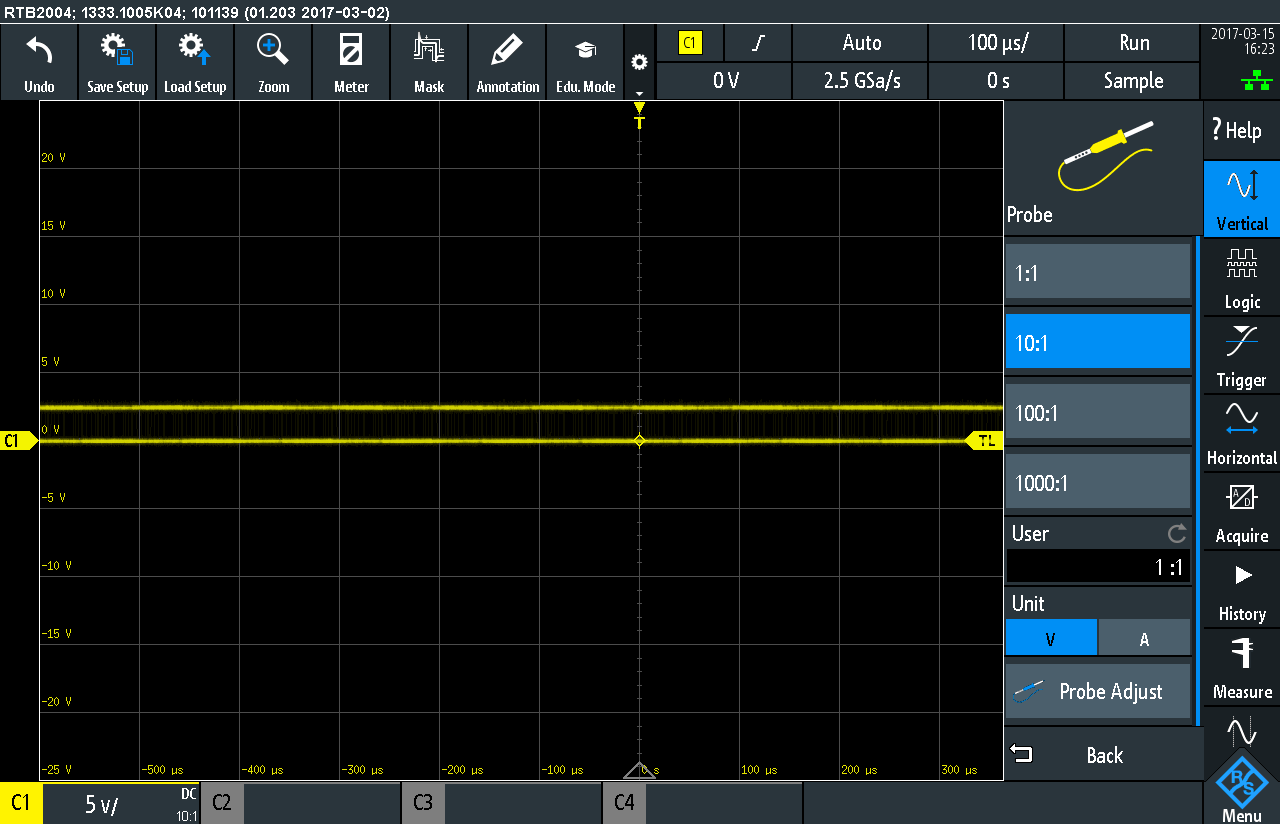
\includegraphics[scale=0.25]{SCR03}
	\caption{Innstillinger for probe på oscilloskop.}
	\label{fig:inst1}
\end{wrapfigure}

Vi kobler om de fire stiftlistparene for å sjekke om de korresponderer med Tabell \ref{tab:abs1}. Nå følger vi med på de to 7-segmentsdisplayene INN og UT for å se input og output. Etter at vi har testet alle verdiene og er overbevist om at kretsen fungerer, kan vi gå videre.

\subsubsection{Oppsett av Oscilloskopet og justering av probe}
Vi vil nå bruke en probe og oscilloskopet til å ta målinger av kretsen. Før vi setter i gang med det, vil vi forsikre oss om at der ikke er brudd i proben vi bruker. Vi følger prosedyren beskrevet i Labratorieheftets vedlegg C.4.1. Vi setter også oscilloscopet til standardinnstillinger ved å trykke på «Preset». Vi setter proben og innstillingen i kanalmenyen på oscilloskopet i modusen 10x som vist i Figur \ref{fig:inst1}.

\subsubsection{Forplantlingsforsinkelse}
For å kunne se hvordan kretsen fungerer når inn- og utverdiene forander seg vil vi koble på signalgeneratoren. Vi gjorde dette ved å koble signalgeneratonen til både oscilloskopets kanal 3 og kretsen ved hjelp av et BNC T-ledd. Vi kobler proben til enden av kritisk sti slik at vi kan måle forplantninsforsinkelsen. Signalgeneratoren ble satt til 100kHz firkantpuls. Spenningen ble satt til 5Vp-p med en offset på 2.5V.

Vi leser av forplantningsforsinkelsen til å være 640 ns. Sammenlignet med utregningene i forarbeider som var på 655ns er det et akseptabelt avvik på 4\% som hovedsaklig stammer fra usikkerhet i målingene våre, men også usikkerheter i komponenter og ledninger.

Med denne informasjonen kan vi regne ut den maksimale klokkefrekvensen for den målte verdien:

\begin{equation}
	f_{max} = \frac{1}{640ns} = 1,56 MHz
\end{equation}

Vi vil så se hva som skjer om vi øker klokkefrekvensen over den maksimale klokkefrekvensen.

\begin{figure}[h]
	\centering
	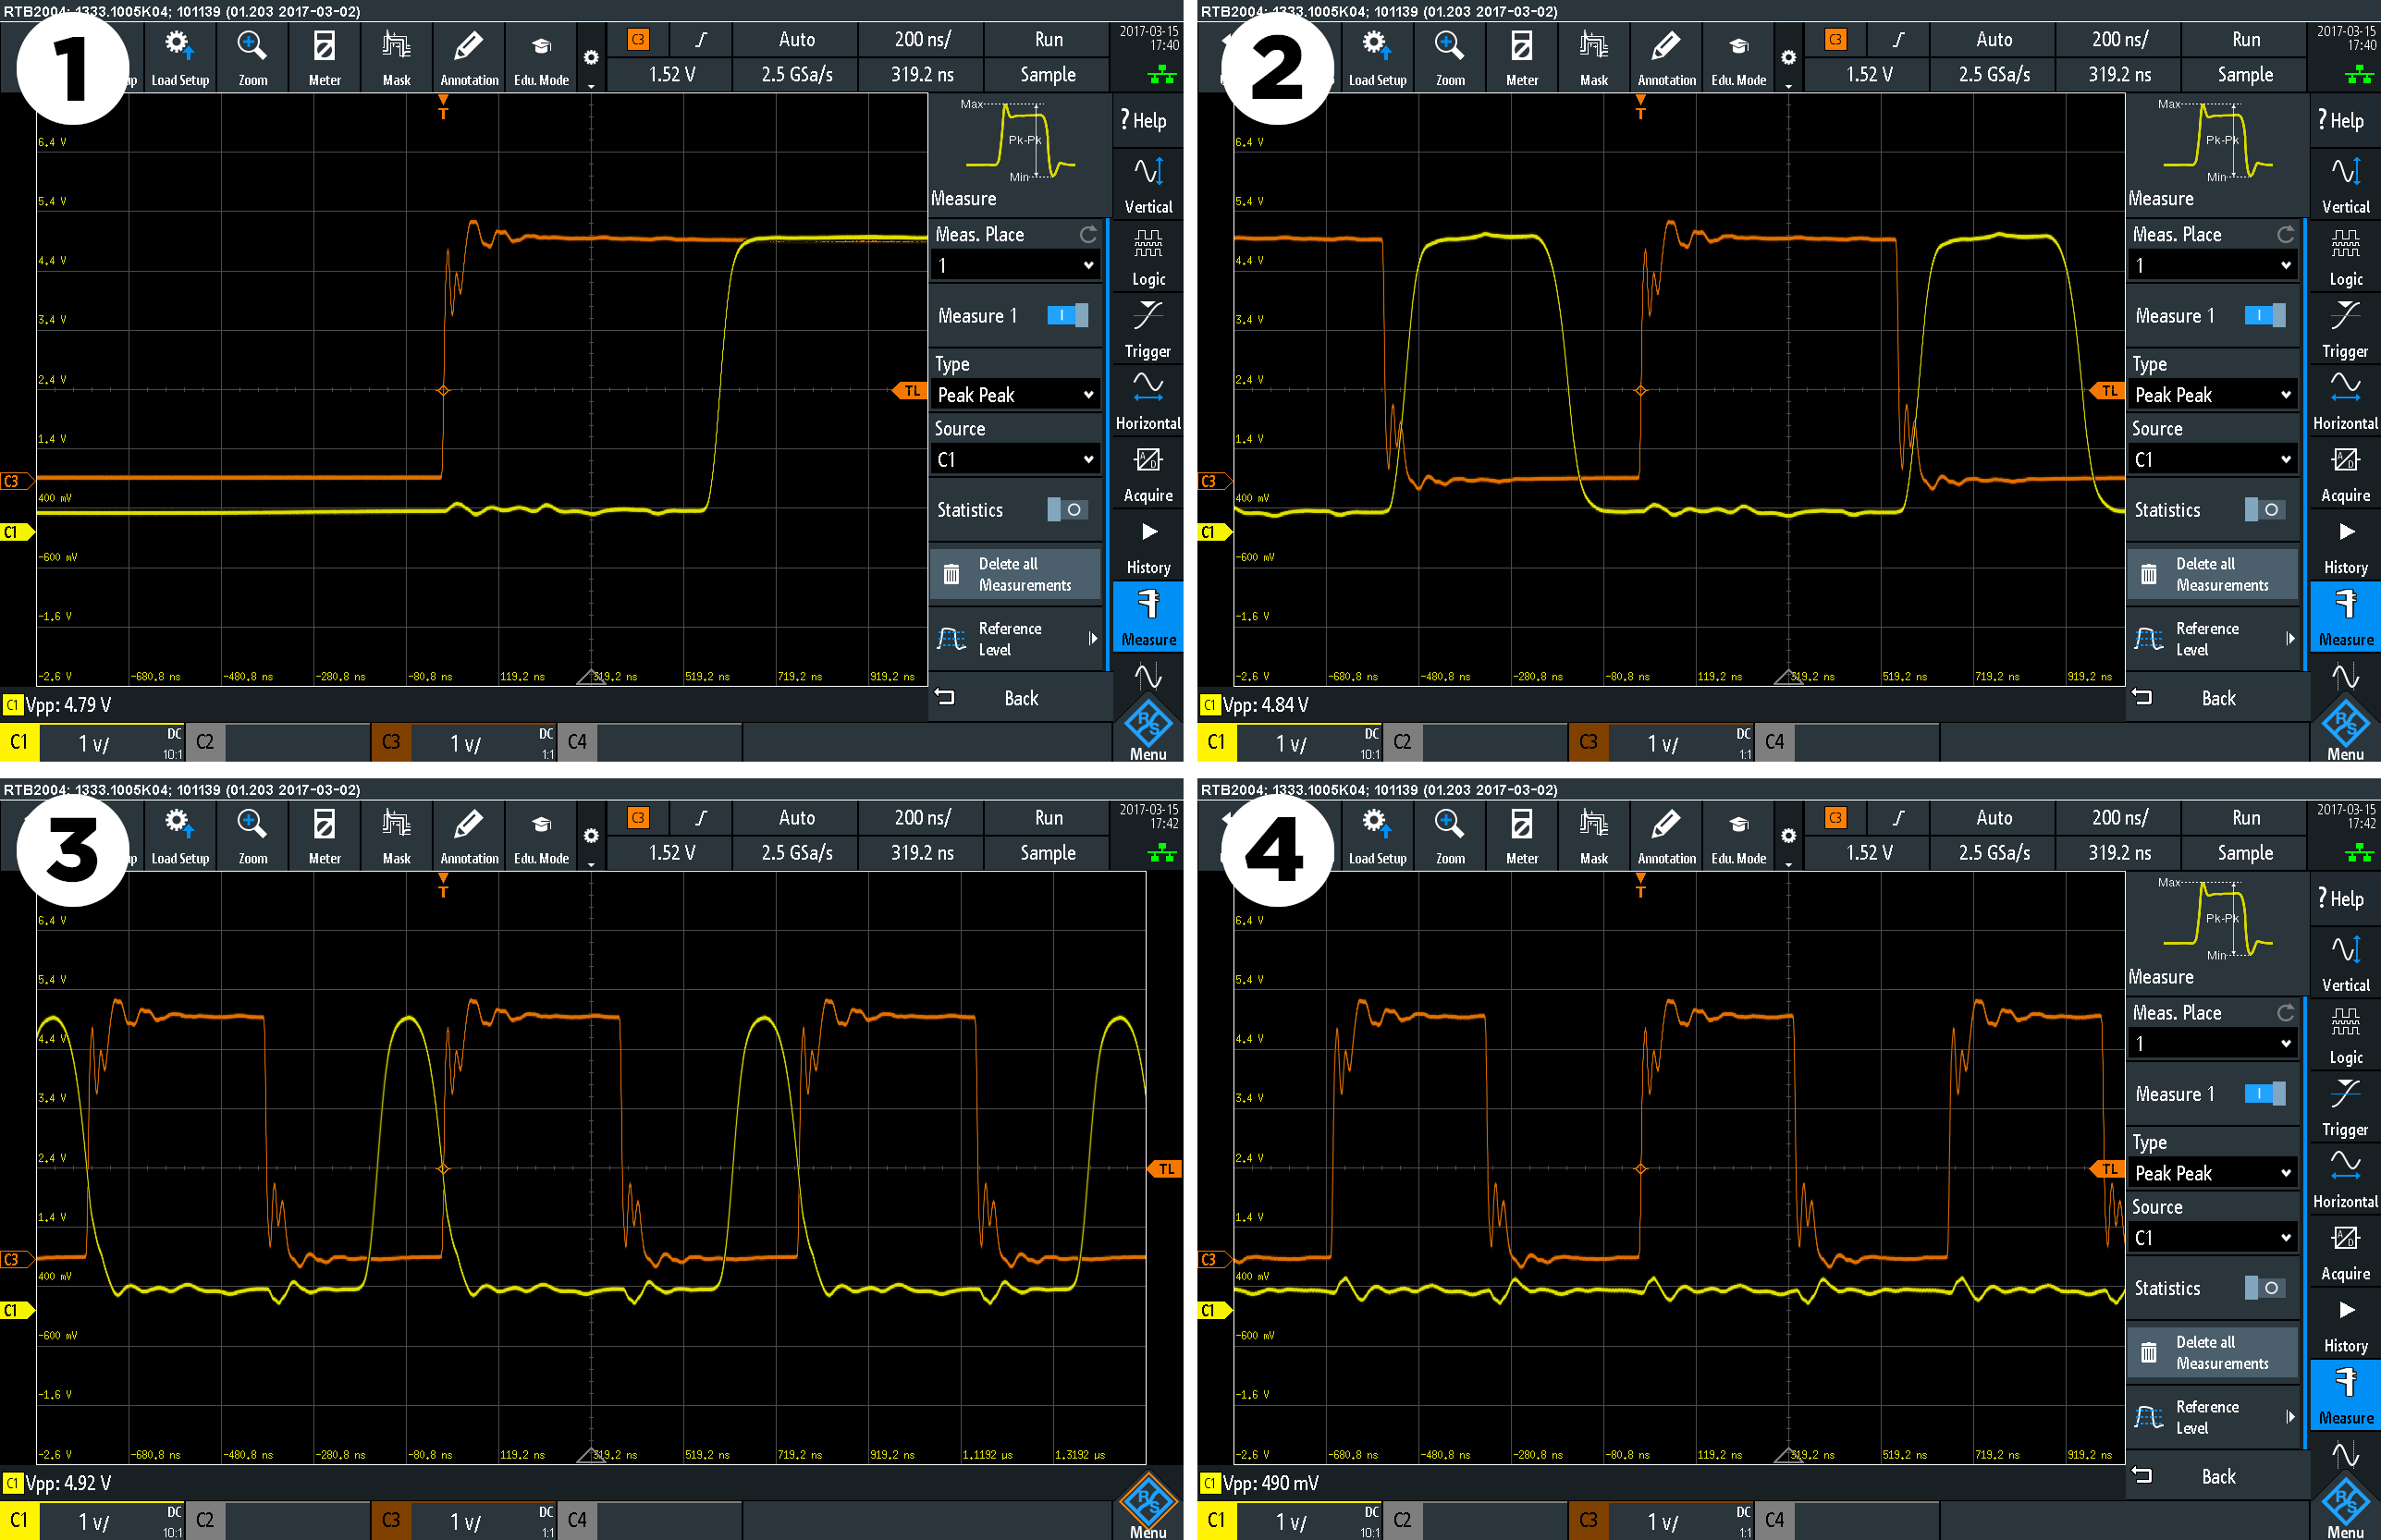
\includegraphics[width=1\linewidth]{tegneserie1}
	\caption{Skjermdump av målingene med varierende frekvens}
	\label{fig:tegneserie1}
\end{figure}

På figur \ref{fig:tegneserie1} ser man skjermdump fra oscilloskopet. Den gule linjen (CH1) beskriver stige- og falltiden til kretsen sin kritiske sti. Den oransje linjen (CH3) kommer rett fra signalgeneratoren gjennom en BNC-BNC kabel.

Vi ser at når vi økte frekvensen vil den på et punkt være så høy at ut signalet hele tiden er lavt. Dette ser man på bilde 3 og 4 i figur \ref{fig:tegneserie1}.

Målingen som ble gjort var å måle stige og falltid for den kritiske stien. Først frem til AND-porten og deretter frem til XOR porten i samme halvadder. Se resultater.


\subsubsection{Stige-/falltid}
Oscilloskopet ble stilt inn til å kun vise en flanke.
% TODO: Laboppgave 5

\section{Utsyrsliste}
Følgende utstyr ble brukt under labben;
\begin{itemize}
	\item Labkort (se % TODO
	\item Ca. 20 ledninger
	\item Probe
	\item Digitalt oscilloskop: Rohde \& Schwarz, RTB2004
	\item Strømforsyning: Rohde \& Schwarz, HMC8042
	\item Signalgenerator: Rohde \& Schwarz, HMF2525
	\item Probe: Rohde \& Schwarz, RT-ZP03
	\item BNC-BNC kabel
	\item BNC T-ledd
\end{itemize}

\section{Resultater}
\begin{table}[h]
	\centering
	\caption{Resultater}
	\label{my-label}
	\begin{tabular}{lllll}
	\textbf{Måling}          & \textbf{Beregnet} & \textbf{Målt} & \textbf{Avik} & \textbf{Avik (\%)} \\
	Forplantningsforsinkelse & 655ns             & 640ns         & 15ns          & 2.3\%              \\
	Rise time                &                   & 47ns          &               &                    \\
	Fall time                &                   & 63ns          &               &                    \\
	Rise time, XOR port      &                   & 32ns          &               &                    \\
	Fall time, XOR port      &                   & 82ns          &               &
	\end{tabular}
\end{table}

\section{Diskusjon}

\section{Konklusjon}

\section{Vedlegg}

\section{Litteraturreferanser}



\end{document}


% \begin{center}
% 	Tabell 1
% \end{center}
% \begin{center} % l = første kollone left, center, right
% 	\begin{tabular} {| l | c | r |} \hline
% 			EN ABS 	& DI 	& DO \\ \hline
% 			4 			& 5 	& $\sqrt{2} + 1$ \\ \hline
% 			7 			& 8 	& 9 \\ \hline
% 	\end{tabular}
% \end{center}
